\chapter{\iflanguage{ngerman}{Steuerung der Robotersysteme}{Control of the robotic systems}}
\label{sec:controlofroboticsystems}
In the last chapter, the feasibility of micro surgeries done with different robotic approaches is shown. But the robotic system is not the only part needed for robot assisted micro surgery. The control of the robotic system is at least as important as the system itself. There are three possible approaches. First the the use of an handheld robotic system, second teleoperation of the system, third the complete automation of the surgery. \\

\subsection{Handheld operation of the robotic system}
\label{sec:handheldoperation}
Handheld robotic systems consists of a robot attached to a hand held controller. The surgeon controls over the handheld the robot. This kind of system is not suitable for miniature robotic systems because accuracy of the system depends on a steady zero point of the robot. This steady zero point is not given when the system is a handheld system because the surgeon has always minimal movement like the tremor of his hands. This movement adds up to a high deviation from the initialized zero point.

\subsection{Teleoperated robotic system}
\label{sec:teleoperation}
Teleoperation is defined as an operation done by a robot controlled over a master console by a human \cite{definition_teleoperation}.  Current systems working this way are for example the Da Vinci System or the Sensei Robotic System. Both are reproducing the  movements at the master end-effector with the follower end-effector. Forces applied to the follower end-effector are reflected at the master end-effector. \\
The surgeon is able to be more precise in his movements because it is not necessary to imitate the surgeon movement 1 to 1. For example if the surgeon moves his tool 1mm to the right the follower end-effector is only moved by 0.1mm. Another feature of teleoperated systems is the tremor of the surgeons hand can be removed with software resulting in a more stable tool movement. These two points are especially important when doing a micro surgery like an eye surgery. For example manually injecting a fluid in a retinal vein which is only 100\textmu m thick is not possible. But a study has shown that it is possible with a teleoperated robotic system \cite{veincannulation}. The next advantage is the point of motion is the wrist of the surgeon in a manually surgery. With teleoperated systems the point of motion can be placed closer to the the organ allowing more freedom in movement.  The fourth point for teleoperated system is the distance independence. A surgeon has no longer to be in the same room as the patient which allows for more collaborations between different hospitals. The collaborations are very important for micro surgeries because the area of micro surgeries is a new area for many surgeries and it requires a high skill of using the tools. There are not many micro surgeons so it is helpful that a hospital only requires the robotic system but a surgeon from another hospital can do the surgery. \\
One issue with the teleoperated tool is the missing redundancy when for example unexpected obstacles are encountered or one of the surgeons team collides with the body or the robot. A collision of the robotic system with a participant moves the zero point of the robotic system without recalibrating the robot resulting in false movement. That's very dangerous in micro surgeries because when the tool tip is only 2mm wide and the zero point was moved by 1mm so the robot is too 50\% in the wrong position. To counter this issue a new control algorithm was evaluated by a team from Milano \cite{redudancy_teleoperation}. The new controller is now able to hold its zero point when a nurse collides with the robot.\\
\newpage
If the surgeon operates manually on the patient he will be able too see something directly and he also feels the resistance of his tools. This haptic feedback is necessary for the surgeon. The tool tip needs to be able to gather the cutaneous (tactile) and the kinesthetic (force) information to provide the surgeon at the master console haptic feedback. Currently, the measuring and representation of the force feedback is possible and also used in devices like the PHANTOM from SensAble Technologies but \grqq tactile devices are not yet commercially available \grqq \cite{force_feedback}. \\
There are different methods for force sensing. The easiest and currently common way is measuring it visually. This method is not accurate enough to emulate the same experience as manually performed on the master console when dealing with images of a 3mm x 3mm size. For true bilateral telemanipulation, accurate sensors which are built into the tool with a high degrees freedom are needed. When designing the sensor, it must be considered that they have to be inexpensive, biocompatible and also sterilizable \cite{force_feedback}. A current topic of the research of Zhan Fan Quek et. al. is to measure the tactile feedback and to build an interface for it \cite{tactile_feedback}. Their work concentrates on skin deformation. They used devices providing cutaneous normal force and skin stretch feedback. Their study shows using tactile feed reduces the applied force. The study participants felt more aware of the situation with the tactile feedback. The participants reported the feedback does not affect their concentration on the task. \\
One great advantage of teleoperated systems is  the surgeons input can be processed with software. The software provides many possibilities for increasing the accuracy and safety of a surgery. Removing tremor was already mentioned but also more advances techniques are possible. One of the biggest dangers is to damage healthy tissue. A team from Tokyo proposed an algorithm to autonomously avoid collisions in robotic neurosurgery \cite{collisionAvoidanceNeuro}. The researcher developed an master-slave neurosurgical robot (MM-3) in a prior work \cite{MM3}. The aim was to develop a teleoperated robot to remove brain tumors in deep and narrow spaces. Therefore a endoscopic or a microscopic view is required. These systems are restricting the view of the surgeon which increases the risk of collisions between surrounding tissue and the tool shaft. To simplify the calculations they modelled the workspace as a truncated cone (Fig. \ref{fig:workspace_model}). Before the surgery starts the opening and the bottom of the workspace are traced. When the shaft gets near the cone the system enters the collision avoidance mode. Then a new shaft position is calculated to avoid a collision. The new position is applied without changing the position of the tool tip (Fig. \ref{fig:reposition}).
\begin{figure}[H]
    \centering
    \begin{subfigure}[b]{0.3\textwidth}
        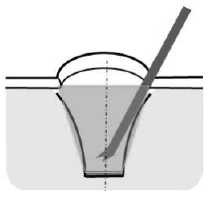
\includegraphics[width=\textwidth]{Figures/workspace_model.png}
        \caption{The workspace volume can be simplified as a truncated cone
beginning in the surface of the brain, and ending in the deep treatment region}
        \label{fig:workspace_model}
    \end{subfigure}
    \qquad \qquad
    \begin{subfigure}[b]{0.3\textwidth}
        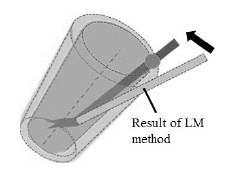
\includegraphics[width=\textwidth]{Figures/collision_avoidance.png}
        \caption{Applied collision avoidance mode. Tool tip position doesn't change when the the tool shaft is repositioned}
        \label{fig:reposition}
    \end{subfigure}
    \caption{Collision avoidance mode \cite{collisionAvoidanceNeuro}}
    \label{fig:collisionavoidancemaode}
\end{figure}
 
\newpage
\subsection{Automatic operated robotic system}
\label{sec:automaticoperation}
The automated collision avoidance algorithm is the first step into the direction of a fully automated micro surgery. Despite, the work on automated surgeries began back in 1988, when a team used an Unimation Puma 200 robot and a CT image of the brain for an automated biopsy operation of the brain \cite{automatedBrainSurgery1988}. This approach of image-guided automated surgical robots (IGASR) was harder to deploy in hospitals because it depends on intraoperative images. For micro surgeries images with a size of around 10mm x 10mm and with a very high resolution are required. This obstacle is getting eliminated by current research \cite{ImagingTechniques}.  \\
A time consuming preoperative step (segmentation and trajectory planning) is often needed for a minimally invasive surgery, especially for surgeries of the temporal bone. A group form the TU Darmstadt tried to automate this step. They use an preoperative CT scan as input for an pipeline consisting of determining the organs at risk and to extract surface models. With this data they calculate the best access points and trajectories to the cochlea and the internal audiotory canal. They used 2D segmentation because 3D labeled data was not yet created. Their work shows that the complete automatic method outperforms the semi automatic approach \cite{PreoperativeStep}. The next step is using the data from the preoperative step to automatically perform the surgery. Their developed pipeline can be modified and retrained to fit other use cases like the planning of a heart surgery.\\
Completely automatic retinal surgeries are not yet possible. However, there are robot assisted approaches. During the retinal surgery the surgeon needs to handle his tools as well as observing them through a microscope. A team from USA, Germany and Italy developed a real time algorithm to track the instruments and also provide the possibility of detection failure. Their detection algorithm is able to (re-)initialize itself \cite{retinal_tool_detector} and to present the detection results to the surgeon. A real time tool tip detection algorithm not only helps the surgeon. It is also needed for the automation of the surgery because the location of the tool tip must always be known during a surgery. This algorithm provides redundancy to the the location calculation by knowing the different parameters of the robot. An image with a high resolution and a very accurate detection algorithm is needed that it is useful for fully automated micro surgeries. Many computer scientist are working on improving detection algorithms. \\
There are many advantages of fully automated micro surgeries over teleoperated surgeries. Once the control of a robot is trained it can be replicated quickly and used anywhere with the same robot. A micro surgeon does need multiple thousands hours of training till he is ready for surgeries on a real patient. A micro surgeon has to learn new techniques during his whole career. The surgeon needs to go to conferences or other meetings with colleagues. The robotic systems can learn in every surgery like a real surgeon but the robots can, if connected to the internet, exchange the findings nearly instantly. If one robot learns how to overcome a certain complication every other robot is also able to overcome this complication. In a new field like the micro surgery not all complications are documented and known by every surgeon.\\
Another advantage is the robots are not depending on a daily mood. Also the concentration of the surgeon is not steady. It depends on the daytime and many other factors. When operating on a micro to millimeter scale a continuous high concentration is a key feature for a successful surgery. This dependency on concentration is completely removed when using a fully automated system. The system can work day and night with the same accuracy.
